% (c) 2002 Matthew Boedicker <mboedick@mboedick.org> (original author) http://mboedick.org
% (c) 2003-2007 David J. Grant <davidgrant-at-gmail.com> http://www.davidgrant.ca
% (c) 2008 Nathaniel Johnston <nathaniel@nathanieljohnston.com> http://www.nathanieljohnston.com
%
% (c) 2012 Scott Clark <sc932@cornell.edu> cam.cornell.edu/~sc932
%
%This work is licensed under the Creative Commons Attribution-Noncommercial-Share Alike 2.5 License. To view a copy of this license, visit http://creativecommons.org/licenses/by-nc-sa/2.5/ or send a letter to Creative Commons, 543 Howard Street, 5th Floor, San Francisco, California, 94105, USA.

\documentclass[letterpaper,11pt]{article}
\newlength{\outerbordwidth}
\pagestyle{empty}
\raggedbottom
\raggedright
\usepackage{xcolor} %Was \usepackage[svgnames]{xcolor}
\usepackage{framed}
\usepackage{tocloft}
\usepackage{enumitem}
\usepackage[hidelinks]{hyperref}




\usepackage{graphicx} 
\usepackage{eso-pic}
\usepackage{tikz}
\usepackage{tikzpagenodes}
\usepackage{tcolorbox}
\tcbuselibrary{skins}
\usetikzlibrary{calc}


%-----------------------------------------------------------
%Edit these values as you see fit

\setlength{\outerbordwidth}{3pt}  % Width of border outside of title bars
% \definecolor{shadecolor}{gray}{0.75}  % Outer background color of title bars (0 = black, 1 = white)
% \definecolor{shadecolorB}{gray}{0.93}  % Inner background color of title bars

% Trying out new colors
\definecolor{myGreen}{RGB}{97, 191, 97}
\definecolor{myPurple}{RGB}{102, 0, 204}

%-----------------------------------------------------------
%Margin setup

\setlength{\evensidemargin}{-0.5in} %Was -0.25in
\setlength{\headheight}{0in}
\setlength{\headsep}{0in}
\setlength{\oddsidemargin}{-0.5in} %Was -0.25in
\setlength{\paperheight}{11in}
\setlength{\paperwidth}{8.5in}
\setlength{\tabcolsep}{0in}
\setlength{\textheight}{10in} %Was 9.5in
\setlength{\textwidth}{7.5in} %Was 7in
\setlength{\topmargin}{-0.8in} %Was -0.3in
\setlength{\topskip}{0in}
\setlength{\voffset}{0.1in}


%-----------------------------------------------------------
%Custom commands
\newcommand{\resitem}[1]{\item #1 \vspace{-2pt}}
\newcommand{\resheading}[1]{\vspace{0pt} %was 8pt
  \parbox{\textwidth}{\setlength{\FrameSep}{\outerbordwidth}
    \begin{shaded}
\setlength{\fboxsep}{0pt}\framebox[\textwidth][l]{\setlength{\fboxsep}{3.5pt}\fcolorbox{shadecolorB}{shadecolorB}{\textbf{\sffamily{\mbox{~}\makebox[7.262in][l]{\large #1} \vphantom{p\^{E}}}}}} % Was 4 and 6.762in
    \end{shaded}
  }\vspace{-7pt} %Was -5 this is spacing between main headers and below text
}
% [5] controls the number of elements
% {6.8in} controls the spacing between CMU and the Graduation Date
\definecolor{shadecolor}{gray}{0.75}  % Outer background color of title bars (0 = black, 1 = white)
\definecolor{shadecolorB}{gray}{0.93}  % Inner background color of title bars


\newtcolorbox{mybox}{enhanced, frame hidden, borderline west = {3pt}{0pt}{black},
skin=bicolor,interior style={left color=myGreen!75,right color=white},
arc=0pt,outer arc=0pt, fontupper=\large}

\newcommand{\ressubheading}[5]{
\begin{tabular*}{6.8in}{l@{\cftdotfill{\cftsecdotsep}\extracolsep{\fill}}r}
		\textbf{#1} & {#2} \\
		{#3} \\
		\textit{#4} \\
		\textit{#5} \\
\end{tabular*}\vspace{-6pt}}
%-----------------------------------------------------------

\usepackage{newpxtext}


\begin{document}


\AddToShipoutPicture* %515,738
	{\put(515,738){
\includegraphics[width=2.25cm,height=1.5cm]{logoGreen.png}}}

% \begin{tikzpicture}[remember picture,overlay]
% 	\clip ($(current page text area.north east)!0.64!(current page text area.south east)!.925!(current page text area.north west)$)
% 		circle (1.5cm) node {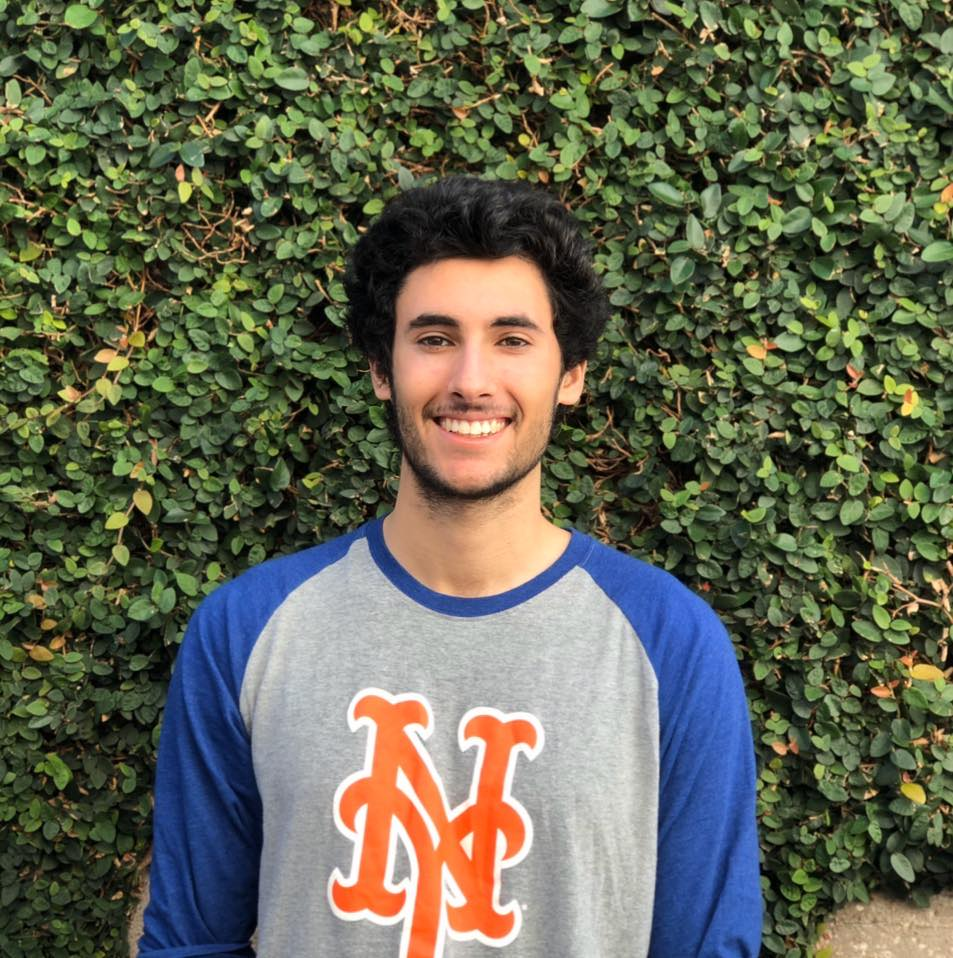
\includegraphics[width=0.2\linewidth]{myPic.jpg}};
% 	\end{tikzpicture}
\begin{tikzpicture}[remember picture,overlay]
	\clip ($(current page text area.north east)!0.75!(current page text area.south east)!.95!(current page text area.north west)$)
		circle (0.87cm) node {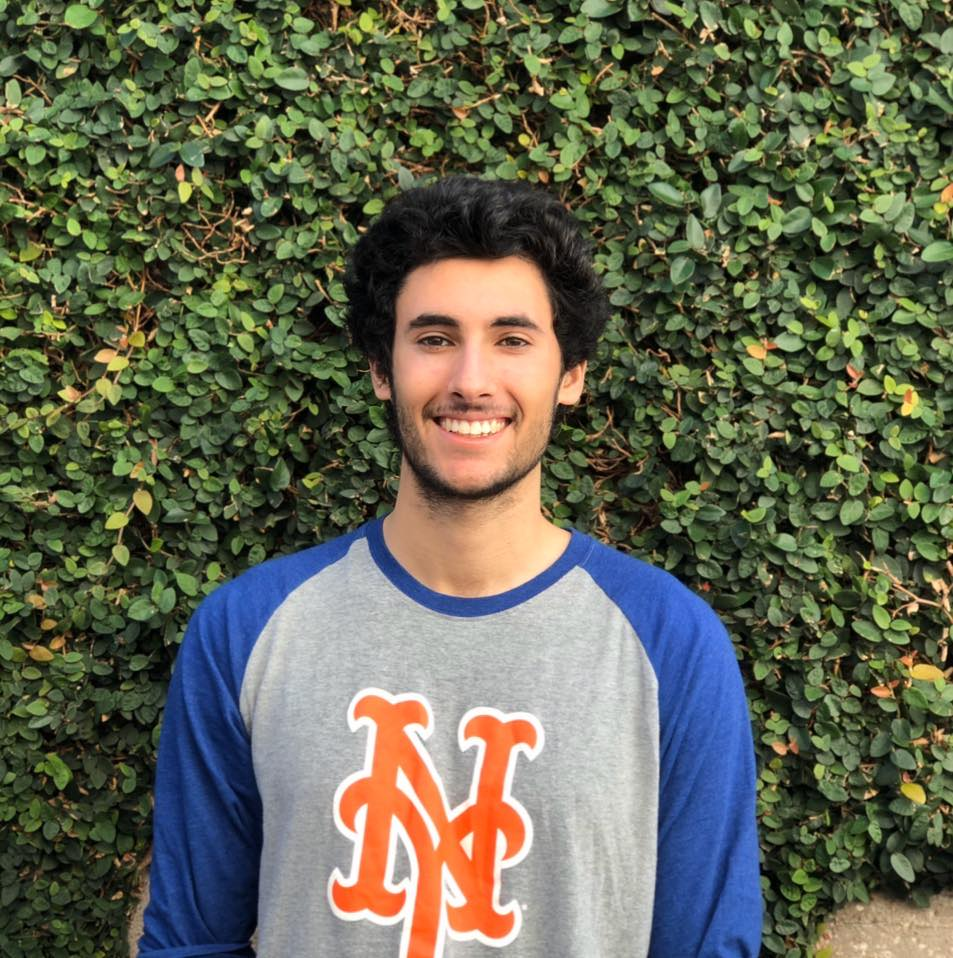
\includegraphics[width=0.125\linewidth]{myPic.jpg}};
	\end{tikzpicture}


\hspace{0.825in} \textbf{\huge Michael E.} \\
\vspace{6pt}
\hspace{0.825in} \textbf{\Huge \textcolor{myGreen}{Kronovet}}

% was 7.45in
%\begin{tabular*}{5.5in}{l@{\extracolsep{\fill}}r}
%\textbf{\Large Michael Kronovet} \\
%\hspace{2in} \href{https://github.com/Mochael}{Github: Mochael} & \href{https://michaelkronovet.com}{michaelkronovet.com} \\
%\hspace{2in} \href{https://www.linkedin.com/in/michael-kronovet}{LinkedIn: michael-kronovet} &  mkronove@andrew.cmu.edu \\
\vspace{-0.45in}  %5.2 to 4.8 and 4.29
\hspace{4.05in} \raisebox{5pt}[\height][\depth]{\href{https://michaelkronovet.com}{\textbf{\LARGE \textcolor{myGreen}{michaelkronovet.com}}}} \\
% \vspace{0.01in}
\hspace{3.9in}  \raisebox{-4pt}[\height][\depth]{\textbf{\LARGE mkronovet@gmail.com}} \\
% \vspace{0.05in}
%\end{tabular*}
%\\

%\itemsep0em USED FOR SPACINIG BETWEEN LINES
%%%%%%%%%%%%%%%%%%%%%%%%%%%%%% 
% \resheading{Education}
\begin{mybox}
	\hspace{-8pt} \textbf{Education}
\end{mybox}
%%%%%%%%%%%%%%%%%%%%%%%%%%%%%%
%\begin{itemize}[leftmargin=10]

%\ressubheading{Carnegie Mellon University}{May 2021}{GPA: 3.77}{Majors in Statistics and Machine Learning, Business Administration}{Minors in Computer Science, Robotics}

\vspace{-10pt}
\begin{enumerate}[leftmargin=10pt]

	\item[] \textbf{Carnegie Mellon University} \cftdotfill{\cftdotsep} August 2017 -- May 2020\\
	GPA: 3.76/4.00 \\
	%\textit{Masters TBD} \\
	\textit{Bachelor of Science in Statistics and Machine Learning with University Honors} \\
	\vspace{-0.3pt}
	%Moneythink Mentor Lead, Joint Funding Committee, APO Service Group \\
	\item[] \textbf{Relevant Courses} \\
	Intro to Machine Learning (PhD), Probabilistic Graphical Models (PhD), Causal Inference (PhD), Algorithms and Advanced Data Structures \\
	\vspace{-0.01pt}
	
\end{enumerate}

%\end{itemize}
%\vspace{-8pt}
\vspace{-10pt}

% \resheading{Work Experience}
\begin{mybox}
	\hspace{-8pt} \textbf{Work Experience}
\end{mybox}

\vspace{-6pt}
\begin{enumerate}[leftmargin=10pt]
	\item[] \textbf{Machine Learning Engineer at \textcolor{myGreen}{Curia.ai}} \cftdotfill{\cftdotsep} August 2020--\\
	\vspace{-4pt}	
	\begin{itemize}
		\resitem{Researched, designed, and implemented the core machine learning backend for all of Curia's products.}
		\resitem{Had a variety of responsibilities including causal inference research, maintaining production models/pipelines, cloud infrastructure, and client facing analysis.}	
	\end{itemize}
	 
	\item[] \textbf{Bioinformatics Intern at \textcolor{myGreen}{Regeneron}} \cftdotfill{\cftdotsep} June 2020 -- August 2020\\
	\vspace{-4pt}	
	\begin{itemize}
		\resitem{Made a machine learning model to predict the exon skipping efficiency of antisense-oligonucleotides (ASOs) and then built a corresponding app to recommend optimal ASOs for specific exon skipping tasks.}	
	\end{itemize}

	\item[] \textbf{Teaching Assistant for \textcolor{myGreen}{10-701 Intro Machine Learning (PhD)}} \cftdotfill{\cftdotsep} January 2020 -- May 2020\\
	\vspace{-4pt}
	\begin{itemize}
		\resitem{Led recitations, created homework problems, held office hours, and advised final projects for the PhD version of the intro to machine learning class at Carnegie Mellon.}
	\end{itemize}

	\item[] \textbf{Data Scientist with \textcolor{myGreen}{Ikos}} \cftdotfill{\cftdotsep} August 2019 -- December 2019\\
	\vspace{-4pt}	
	\begin{itemize}
		\resitem{Built and later sold (to Ikos) an app that would predict how much property rentals across Pittsburgh would rent for and how quickly they would rent.}	
	\end{itemize}
	
	\item[] \textbf{Quantitative Trading Intern at \textcolor{myGreen}{Virtu Financial}} \cftdotfill{\cftdotsep} June 2019 -- August 2019\\
	\vspace{-4pt}
	\begin{itemize}
		\resitem{Worked on the algorithms team at a high frequency trading firm to predict Exchange Traded Fund (ETF) price fluctuations and alter trading strategies to profit from them.}
	\end{itemize}
\end{enumerate}

\vspace{-10pt}
%\vspace{-6pt}

%%%%%%%%%%%%%%%%%%%%%%%%%%%%%%
% \resheading{Projects}
\begin{mybox}
	\hspace{-8pt} \textbf{Projects}  \fontsize{10.5}{15}\selectfont   (A more extensive list is on my website)
\end{mybox}

% \textbf{\textcolor{myGreen}{Learn more about my projects on}} \hspace{-6pt} \href{https://michaelkronovet.com}{\textbf{ \textcolor{myGreen}{michaelkronovet.com}}}

%%%%%%%%%%%%%%%%%%%%%%%%%%%%%%
\vspace{-5pt}
\begin{enumerate}[leftmargin=10pt]
\setlength\itemsep{1em}

\item[] \href{https://whim.so/}{\textbf{Whim}}\\
\vspace{-4pt}
\begin{itemize}
	\resitem{Building a lightweight, markdown WYSIWYG note taking app that is designed to help you write modular notes which reference each other to aid with knowledge retention. Learn more on \href{https://whim.so/}{Whim.so.}}
\end{itemize}

\vspace{-12pt}

\item[] \textbf{Databased Perspectives}\\
\vspace{-4pt}
\begin{itemize}
	\resitem{Creating a website that serves as both a repository for political datasets and as a blog where statistical techniques are applied to analyze government policies.}
\end{itemize}

\vspace{-12pt}

\item[] \textbf{Time Varying Graphs with NOTEARS}\\
\vspace{-4pt}
\begin{itemize}
	\resitem{Adapted a state of the art DAG structure estimation algorithm to build dynamic bayesian networks with time series data.}
\end{itemize}

\end{enumerate}

%\vspace{-6pt}
\vspace{-10pt}

% \resheading{Skills}
\begin{mybox}
	\hspace{-8pt} \textbf{Skills}
\end{mybox}

\vspace{-5pt}
	\begin{enumerate}[leftmargin=10pt]
		\itemsep0em
		\item[] \textbf{Languages/Frameworks}: Python, R, SQL, Javascript, Typescript, React, Django, Jekyll, C, Matlab
		\item[] \textbf{Technologies}: Git, Docker, Spark, AWS, GCP, Figma, CAD, Unity, Microsoft Excel
		
	\end{enumerate}

\end{document}